\documentclass[10pt]{report}

\usepackage[utf8]{inputenc}
\usepackage[vietnamese]{babel}

\usepackage{float}
\usepackage{graphicx}
\usepackage{tabularx}
\usepackage{booktabs}
\usepackage{geometry}
\geometry{a4paper, portrait, margin=25mm, bmargin=25mm, tmargin=25mm}
\setlength{\parskip}{1em}

\usepackage{titlesec}
\titleformat{\chapter}[block]{\normalfont\huge\bfseries}{\thechapter.}{1em}{\Huge}
\titlespacing{\chapter}{0pt}{0pt}{5pt}
\titlespacing{\section}{0pt}{5pt}{5pt}

\usepackage{hyperref}
\hypersetup{
    colorlinks=true,
    linkcolor=blue,
    filecolor=magenta,
    urlcolor=cyan,
}

\begin{document}
\begin{titlepage}
	\centering
	\vspace*{0.5cm}
	\LARGE{Đại học Quốc gia thành phố Hồ Chí Minh}\\[-0.2ex]
	\LARGE{Trường Đại học Công nghệ Thông tin}\\[2.5ex]
	\large{Khoa Khoa học Máy tính}\\
	\noindent\rule{\textwidth}{0.2pt}\\
	\vspace{2cm}
	
\includegraphics[width=5cm]{assets/uit_logo.eps}\\
	\vspace{2cm}
	\textbf{\LARGE{MẠNG NEURAL VÀ THUẬT GIẢI DI TRUYỀN}}
	\medskip\par
	\textbf{\Large{BÁO CÁO BÀI TẬP SỐ 2}}
	\medskip\par
	\Large{Differential Evolution và Cross Entropy Method}\\[-1.5ex]
	\vspace{0.4cm}
	\noindent\rule{0.5\textwidth}{0.2pt}\\
	\vspace{0.4cm}
	\large{Huỳnh Anh Dũng -- 22520278}\\[-0.2ex]
	\large{Lớp: CS410.P21}\\[-0.2ex]
	\vspace{0.4cm}
	\noindent\rule{0.5\textwidth}{0.2pt}\\
	\vspace{1.6cm}
	\medskip
	\raggedright
	\begin{tabular}{ll}
		Ngày thực hiện:       & ngày 03 tháng 4 năm 2025 \\[-0.2ex]
		Giảng viên hướng dẫn: & thầy Lương Ngọc Hoàng    \\
	\end{tabular}
\end{titlepage}

\tableofcontents
\newpage

\chapter{Giới thiệu}
Bài báo cáo thực nghiệm bài toán tối ưu hóa trên hai thuật toán \emph{Differential Evolution} (DE) và \emph{Cross-Entropy Method} (CEM) nhằm đánh giá tốc độ hội tụ, độ chính xác của lời giải cuối và tính ổn định của giải thuật khi thử nghiệm trên nhiều hàm benchmark khác nhau.

Bộ hàm benchmark sẽ được sử dụng bao gồm:
\begin{itemize}
	\item Hàm \emph{Sphere}: hàm lồi có công thức đơn giản, thường dùng làm tiêu chí tiên quyết của bài toán tối ưu hóa.
	\item Hàm \emph{Griewank}: hàm benchmark có công thức phức tạp tạo nhiều điểm cực tiểu lân cận, gây khó khăn cho việc tìm ra lời giải tối ưu toàn cục.
	\item Hàm \emph{Rosenbrock}: hàm phi lồi với đoạn lũng hẹp và cong dẫn đến điểm cực tiểu toàn cục.
	\item Hàm \emph{Rastrigin}: hàm benchmark có tính đa cực cao nhưng có một lượng lớn các cực tiểu lân cận nằm theo phân bố đều.
	\item Hàm \emph{Ackley}: hàm có nhiều cực tiểu lân cận phân bố đều ở vùng ngoài cùng với một cực tiểu toàn cục tại trung tâm, dễ khiến lời giải của các giải thuật tối ưu mắc kẹt ở một trong những cực tiểu lân cận.
\end{itemize}

Với mỗi bộ tham số thực nghiệm (bao gồm kích thước quần thể, số lượng tham số, hàm benchmark), sinh viên sẽ chạy với 10 random seed \([22520278; 22520278 + 10)\) để đảm bảo tính khách quan của thực nghiệm. Giải pháp tối ưu toàn cục và không gian tìm kiếm (với số lượng tham số bằng 2) với mỗi hàm được tham khảo từ \href{https://www.sfu.ca/~ssurjano/optimization.html}{đường dẫn}.

\begin{table}[H]\centering
	\caption{Miền tìm kiếm được gợi ý và giải pháp tối ưu toàn cục của các hàm benchmark}
	\begin{tabularx}{0.6\textwidth}{XXX}
		\toprule
		\textbf{Hàm} & \textbf{Giải pháp} & \textbf{Miền tìm kiếm} \\
		\midrule
		Sphere       & \((0, 0)\)         & \([-5.12, 5.12]\)      \\
		Griewank     & \((0, 0)\)         & \([-600, 600]\)        \\
		Rosenbrock   & \((1, 1)\)         & \([-5, 10]\)           \\
		Rastrigin    & \((0, 0)\)         & \([-5.12, 5.12]\)      \\
		Ackley       & \((0, 0)\)         & \([-32.768, 32.768]\)  \\
		\bottomrule
	\end{tabularx}
\end{table}

Trong quá trình thực nghiệm, một số siêu tham số của mô hình đã được sinh viên cài đặt như sau:
\begin{itemize}
	\item Với DE: các siêu tham số \texttt{scale\_factor} và \texttt{crossover\_probabilities} được cài đặt lần lượt là 0.7 và 0.5.
	\item Với CEM: siêu tham số \texttt{elites\_size} được cài đặt bằng \(\frac{1}{2}\) của \texttt{population\_size}.
\end{itemize}

\chapter{Kết quả thực nghiệm}
\emph{*Các kết quả thực nghiệm bên dưới đều được làm tròn đến chữ số thập phân thứ 2, \emph{p-value} được làm tròn đến chữ số thập phân thứ 3.}

\emph{**Nếu giá trị \emph{p-value} dưới ngưỡng 0.05 thì kết quả t-test sẽ được coi là có tầm quan trọng.}

\section{Thực nghiệm với hàm benchmark Sphere}
\begin{figure}[H]\centering
	\label{figure:sphere_comparison}
	\caption{Biểu đồ hội tụ của hai thuật toán với hàm Sphere với \(N = 32 \wedge d \in \{2; 10\}\)}
	\begin{minipage}{0.45\textwidth}\centering
		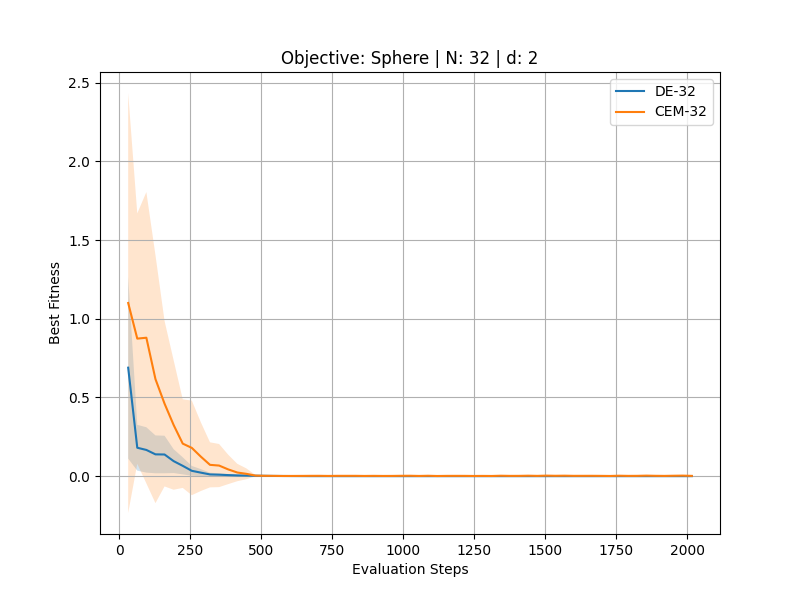
\includegraphics[width=\textwidth]{../assets/graphs/objective=Sphere_N=32_d=2.png}
	\end{minipage}
	\begin{minipage}{0.45\textwidth}\centering
		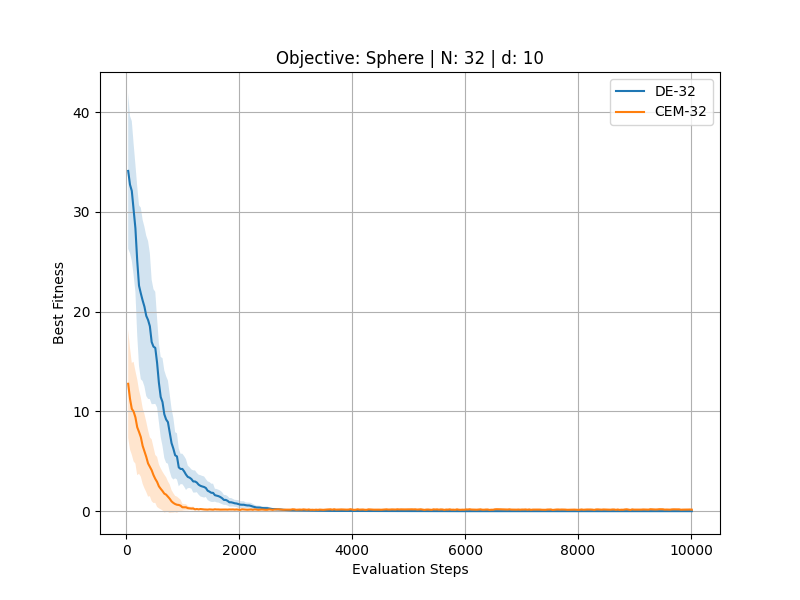
\includegraphics[width=\textwidth]{../assets/graphs/objective=Sphere_N=32_d=10.png}
	\end{minipage}
\end{figure}

\begin{table}[H]\centering
	\caption{Bảng so sánh giải pháp tốt nhất với hàm benchmark Sphere}
	\begin{tabularx}{0.8\textwidth}{p{5em}XXl}
		\toprule
		\textbf{N} & \textbf{DE}              & \textbf{CEM}               & \textbf{p-value}   \\
		\midrule
		\multicolumn{4}{c}{\(d = 2\)}                                                           \\
		\midrule
		8          & \(0.0 \pm 0.0\)          & \(0.0 \pm 0.0\)            & \(\mathbf{0.001}\) \\
		16         & \(0.0 \pm 0.0\)          & \(0.0 \pm 0.0\)            & \(\mathbf{0.004}\) \\
		32         & \(0.0 \pm 0.0\)          & \(0.0 \pm 0.0\)            & \(\mathbf{0.007}\) \\
		64         & \(0.0 \pm 0.0\)          & \(0.0 \pm 0.0\)            & \(\mathbf{0.002}\) \\
		128        & \(0.0 \pm 0.0\)          & \(0.0 \pm 0.0\)            & \(0.52\)           \\
		\midrule
		\multicolumn{4}{c}{\(d = 10\)}                                                          \\
		\midrule
		8          & \(\mathbf{0.0 \pm 0.0}\) & \(0.29 \pm 0.11\)          & \(\mathbf{0.0}\)   \\
		16         & \(\mathbf{0.0 \pm 0.0}\) & \(0.22 \pm 0.08\)          & \(\mathbf{0.0}\)   \\
		32         & \(\mathbf{0.0 \pm 0.0}\) & \(0.15 \pm 0.04\)          & \(\mathbf{0.0}\)   \\
		64         & \(\mathbf{0.0 \pm 0.0}\) & \(0.15 \pm 0.04\)          & \(\mathbf{0.0}\)   \\
		128        & \(0.17 \pm 0.05\)        & \(\mathbf{0.13 \pm 0.03}\) & \(0.053\)          \\
		\bottomrule
	\end{tabularx}
\end{table}

Về tốc độ hội tụ, hình \ref{figure:sphere_comparison} cho thấy DE và CEM có tốc độ hội tụ với hàm Sphere gần ngang nhau khi đồ thị cả hai đều có dạng giảm mạnh ở những bước đầu và ổn định sớm ở gần giá trị cực tiểu toàn cục cho đến hết thực nghiệm.

Về độ ổn định, DE thể hiện vượt trội hơn hẳn khi vùng biểu thị phương sai trên hình \ref{figure:sphere_comparison} đều nhỏ hơn hoặc bằng khi so với CEM.

Về độ chính xác của giải pháp cuối cùng, cả hai không có sự khác biệt quá lớn nhưng DE vẫn nhỉnh hơn CEM khi đa phần các kết quả thực nghiệm của DE đều tốt hơn hoặc bằng CEM, đặc biệt khi số chiều tăng lên 10.

\section{Thực nghiệm với hàm benchmark Rosenbrock}
\begin{figure}[H]\centering
	\label{figure:rosenbrock_comparison}
	\caption{Biểu đồ hội tụ của hai thuật toán với hàm Rosenbrock với \(N = 32 \wedge d \in \{2; 10\}\)}
	\begin{minipage}{0.45\textwidth}\centering
		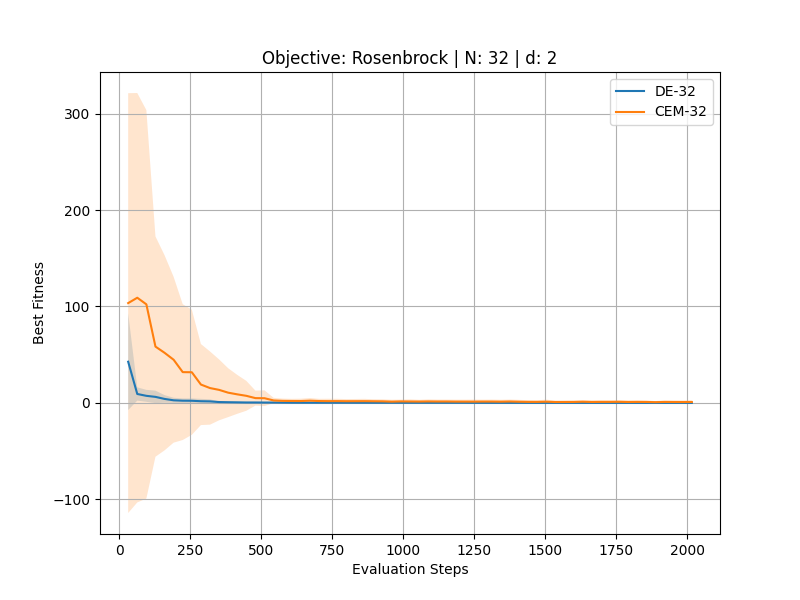
\includegraphics[width=\textwidth]{../assets/graphs/objective=Rosenbrock_N=32_d=2.png}
	\end{minipage}
	\begin{minipage}{0.45\textwidth}\centering
		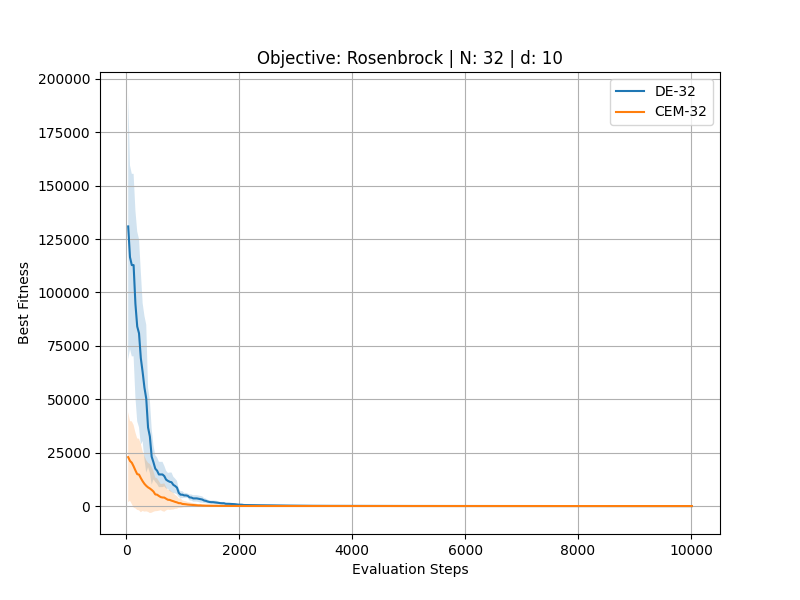
\includegraphics[width=\textwidth]{../assets/graphs/objective=Rosenbrock_N=32_d=10.png}
	\end{minipage}
\end{figure}

\begin{table}[H]\centering
	\caption{Bảng so sánh giải pháp tốt nhất với hàm benchmark Rosenbrock}
	\begin{tabularx}{0.8\textwidth}{p{5em}XXl}
		\toprule
		\textbf{N} & \textbf{DE}                  & \textbf{CEM}                & \textbf{p-value}   \\
		\midrule
		\multicolumn{4}{c}{\(d = 2\)}                                                                \\
		\midrule
		8          & \(\mathbf{0.05 \pm 0.11}\)   & \(1.24 \pm 2.14\)           & \(0.114\)          \\
		16         & \(\mathbf{0.0 \pm 0.01}\)    & \(0.61 \pm 0.6\)            & \(\mathbf{0.007}\) \\
		32         & \(\mathbf{0.0 \pm 0.0}\)     & \(0.97 \pm 1.67\)           & \(0.1\)            \\
		64         & \(\mathbf{0.03 \pm 0.02}\)   & \(0.83 \pm 1.38\)           & \(0.095\)          \\
		128        & \(\mathbf{0.11 \pm 0.15}\)   & \(1.21 \pm 1.81\)           & \(0.088\)          \\
		\midrule
		\multicolumn{4}{c}{\(d = 10\)}                                                               \\
		\midrule
		8          & \(\mathbf{12.56 \pm 20.75}\) & \(35.23 \pm 10.99\)         & \(\mathbf{0.01}\)  \\
		16         & \(\mathbf{4.52 \pm 0.68}\)   & \(25.56 \pm 5.96\)          & \(\mathbf{0.0}\)   \\
		32         & \(\mathbf{7.73 \pm 2.63}\)   & \(21.86 \pm 3.16\)          & \(\mathbf{0.0}\)   \\
		64         & \(41.01 \pm 13.7\)           & \(\mathbf{22.68 \pm 3.1}\)  & \(\mathbf{0.001}\) \\
		128        & \(244.99 \pm 76.76\)         & \(\mathbf{25.0 \pm 16.87}\) & \(\mathbf{0.0}\)   \\
		\bottomrule
	\end{tabularx}
\end{table}

Tốc độ hội tụ của hai thuật toán theo hình \ref{figure:rosenbrock_comparison} là gần như nhau, cả hai đều hội tụ sớm và ổn định tại điểm cực tiểu toàn cục.

Tuy vậy, độ ổn định của DE ở bài toán benchmark này lại vượt trội hơn hẳn so với CEM, khi mà vùng tô màu phương sai theo hình \ref{figure:rosenbrock_comparison} của CEM rất rộng còn với DE lại hẹp đến gần như không có.

Độ chính xác của giải pháp cuối cùng của DE so với CEM nhỉnh hơn đôi phần khi số chiều là 2 nhưng đa phần đều không được ủng hộ khi được kiểm định với giả thuyết thống kê. Ngược lại, kết quả của thực nghiệm với số chiều bằng 10 đều được giả thuyết thống kê ủng hộ và cho thấy giải pháp của DE sẽ chính xác hơn nhưng chỉ với N nhỏ hơn 64; với N bằng 64 hoặc 128, DE không được hiệu quả bằng CEM.

\section{Thực nghiệm với hàm mục tiêu Rastrigin}
\begin{figure}[H]\centering
	\label{figure:rastrigin_comparison}
	\caption{Biểu đồ hội tụ của hai thuật toán với hàm Rastrigin với \(N = 32 \wedge d \in \{2; 10\}\)}
	\begin{minipage}{0.45\textwidth}\centering
		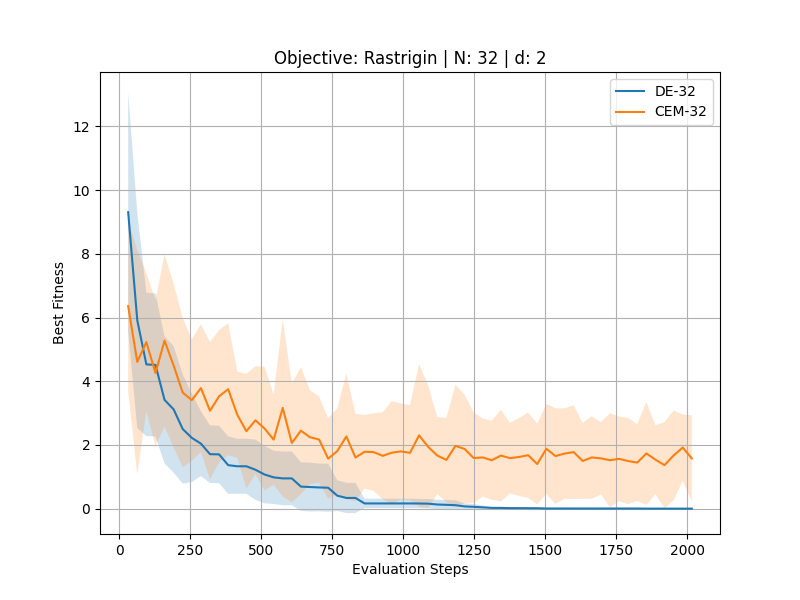
\includegraphics[width=\textwidth]{../assets/graphs/objective=Rastrigin_N=32_d=2.png}
	\end{minipage}
	\begin{minipage}{0.45\textwidth}\centering
		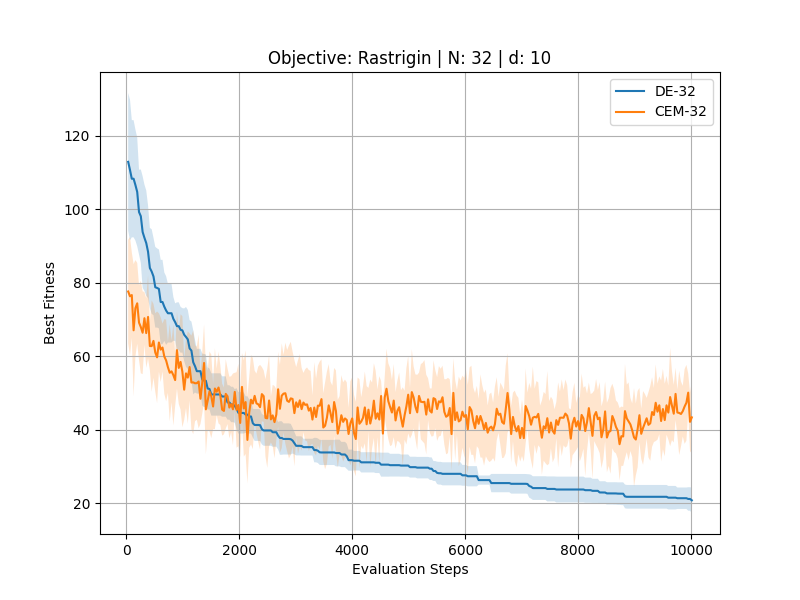
\includegraphics[width=\textwidth]{../assets/graphs/objective=Rastrigin_N=32_d=10.png}
	\end{minipage}
\end{figure}

\begin{table}[H]\centering
	\caption{Bảng so sánh thực nghiệm sử dụng hàm mục tiêu Rastrigin}
	\begin{tabularx}{0.8\textwidth}{p{5em}XXl}
		\toprule
		\textbf{N} & \textbf{DE}                 & \textbf{CEM}        & \textbf{p-value}   \\
		\midrule
		\multicolumn{4}{c}{\(d = 2\)}                                                       \\
		\midrule
		8          & \(\mathbf{0.4 \pm 0.49}\)   & \(4.57 \pm 1.94\)   & \(\mathbf{0.0}\)   \\
		16         & \(\mathbf{0.1 \pm 0.3}\)    & \(3.67 \pm 1.84\)   & \(\mathbf{0.0}\)   \\
		32         & \(\mathbf{0.0 \pm 0.0}\)    & \(1.58 \pm 1.35\)   & \(\mathbf{0.003}\) \\
		64         & \(\mathbf{0.19 \pm 0.16}\)  & \(1.74 \pm 1.57\)   & \(\mathbf{0.008}\) \\
		128        & \(\mathbf{0.46 \pm 0.39}\)  & \(1.28 \pm 0.75\)   & \(\mathbf{0.009}\) \\
		\midrule
		\multicolumn{4}{c}{\(d = 10\)}                                                      \\
		\midrule
		8          & \(\mathbf{4.44 \pm 2.2}\)   & \(64.76 \pm 15.16\) & \(\mathbf{0.0}\)   \\
		16         & \(\mathbf{9.68 \pm 2.99}\)  & \(48.11 \pm 8.71\)  & \(\mathbf{0.0}\)   \\
		32         & \(\mathbf{20.84 \pm 3.46}\) & \(43.39 \pm 9.86\)  & \(\mathbf{0.0}\)   \\
		64         & \(\mathbf{26.78 \pm 4.14}\) & \(40.77 \pm 11.63\) & \(\mathbf{0.003}\) \\
		128        & \(\mathbf{37.62 \pm 4.87}\) & \(43.31 \pm 7.98\)  & \(0.084\)          \\
		\bottomrule
	\end{tabularx}
\end{table}

Tốc độ hội tụ của DE trong bài benchmark Griewank thực sự vượt trội hơn so với CEM vì CEM theo như hình \ref{figure:rastrigin_comparison} vẫn có biên độ dao động khá lớn mặc dù đã đến cuối thời gian thực nghiệm, nên sinh viên nhận định rằng CEM vẫn chưa đạt được mức độ hội tụ tối ưu trong khi DE đã ổn định từ những bước sớm hơn với d = 2 và tiến gần hơn một cách ổn định đến giá trị cực tiểu toàn cục ở cuối thực nghiệm.

Độ ổn định của DE cũng đáng kể hơn khi đồ thị của CEM cho thấy vùng biểu thị phương sai của DE hẹp hơn CEM nhiều.

Tính chính xác của giải pháp cuối cùng vẫn vượt trội hơn về phần DE với mọi điều kiện thử nghiệm và hầu hết đều được ủng hộ bởi kiểm định giả thuyết thống kê.

\section{Thực nghiệm với hàm mục tiêu Griewank}
\begin{figure}[H]\centering
	\caption{Biểu đồ hội tụ của hai thuật toán với hàm Griewank với \(N = 32 \wedge d \in \{2; 10\}\)}
	\begin{minipage}{0.45\textwidth}\centering
		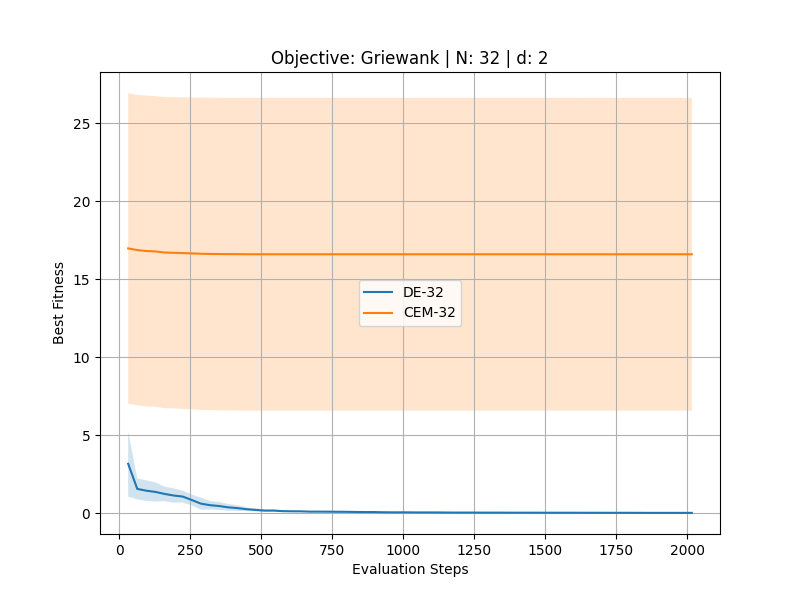
\includegraphics[width=\textwidth]{../assets/graphs/objective=Griewank_N=32_d=2.png}
	\end{minipage}
	\begin{minipage}{0.45\textwidth}\centering
		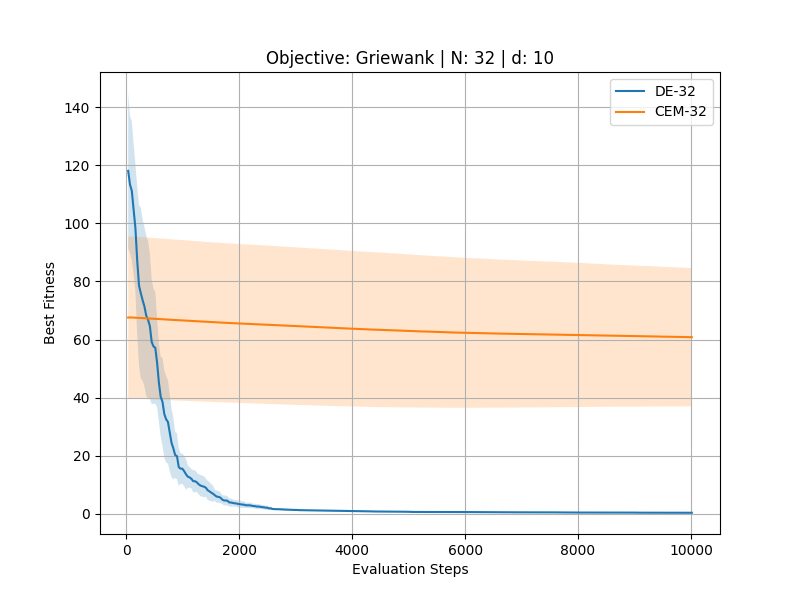
\includegraphics[width=\textwidth]{../assets/graphs/objective=Griewank_N=32_d=10.png}
	\end{minipage}
\end{figure}

\begin{table}[H]\centering
	\caption{Bảng so sánh thực nghiệm sử dụng hàm mục tiêu Griewank}
	\begin{tabularx}{0.8\textwidth}{p{5em}XXl}
		\toprule
		\textbf{N} & \textbf{DE}                & \textbf{CEM}        & \textbf{p-value} \\
		\midrule
		\multicolumn{4}{c}{\(d = 2\)}                                                    \\
		\midrule
		8          & \(\mathbf{0.01 \pm 0.01}\) & \(16.59 \pm 10.02\) & \(\mathbf{0.0}\) \\
		16         & \(\mathbf{0.0 \pm 0.0}\)   & \(16.64 \pm 10.01\) & \(\mathbf{0.0}\) \\
		32         & \(\mathbf{0.02 \pm 0.01}\) & \(16.59 \pm 10.03\) & \(\mathbf{0.0}\) \\
		64         & \(\mathbf{0.04 \pm 0.02}\) & \(16.59 \pm 10.03\) & \(\mathbf{0.0}\) \\
		128        & \(\mathbf{0.07 \pm 0.05}\) & \(16.59 \pm 10.03\) & \(\mathbf{0.0}\) \\
		\midrule
		\multicolumn{4}{c}{\(d = 10\)}                                                   \\
		\midrule
		8          & \(\mathbf{0.06 \pm 0.05}\) & \(47.62 \pm 14.49\) & \(\mathbf{0.0}\) \\
		16         & \(\mathbf{0.21 \pm 0.08}\) & \(54.59 \pm 20.05\) & \(\mathbf{0.0}\) \\
		32         & \(\mathbf{0.35 \pm 0.08}\) & \(60.81 \pm 23.81\) & \(\mathbf{0.0}\) \\
		64         & \(\mathbf{0.62 \pm 0.08}\) & \(63.53 \pm 26.67\) & \(\mathbf{0.0}\) \\
		128        & \(\mathbf{1.57 \pm 0.19}\) & \(64.67 \pm 27.38\) & \(\mathbf{0.0}\) \\
		\bottomrule
	\end{tabularx}
\end{table}

Với bài benchmark Griewank, CEM gần như không có hiệu quả. DE vẫn ổn định nếu không muốn nói là rất phù hợp cho bài toán này.

\section{Thực nghiệm với hàm mục tiêu Ackley}
\begin{figure}[H]\centering
	\caption{Biểu đồ hội tụ của hai thuật toán với hàm Ackley với \(N = 32 \wedge d \in \{2; 10\}\)}
	\begin{minipage}{0.45\textwidth}\centering
		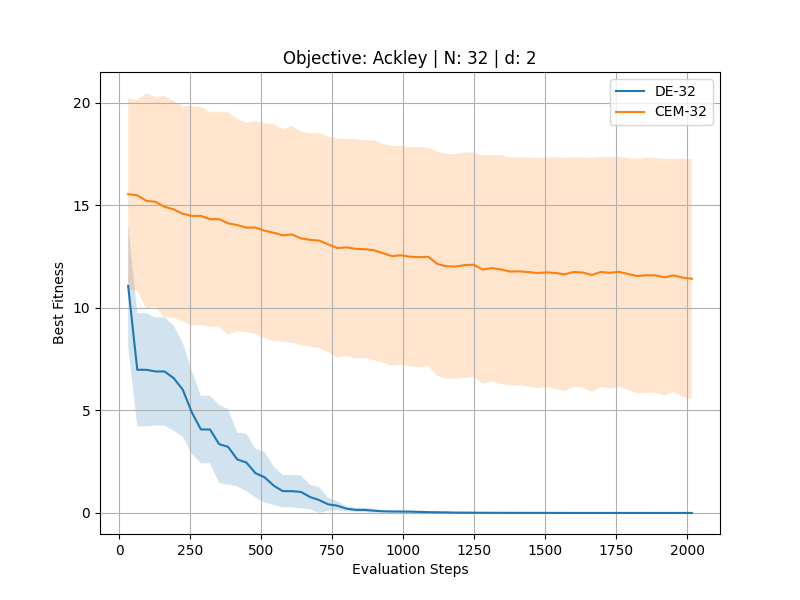
\includegraphics[width=\textwidth]{../assets/graphs/objective=Ackley_N=32_d=2.png}
	\end{minipage}
	\begin{minipage}{0.45\textwidth}\centering
		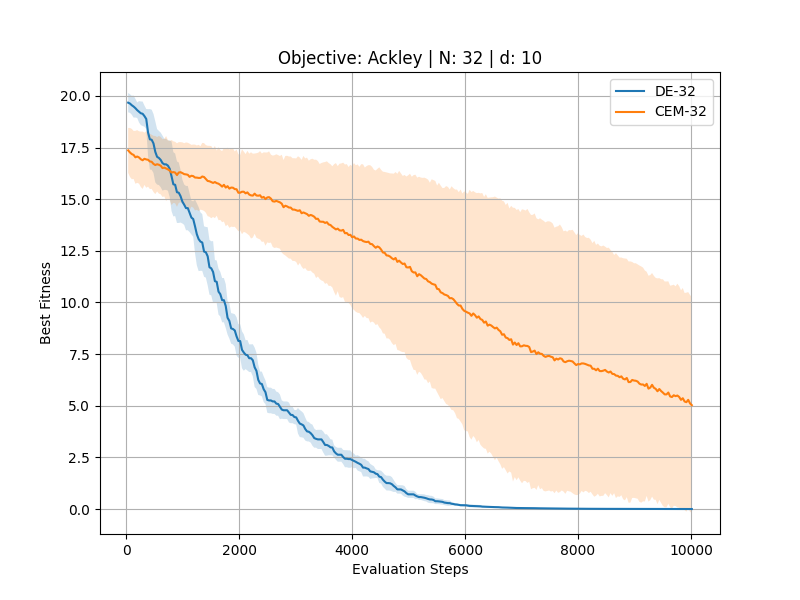
\includegraphics[width=\textwidth]{../assets/graphs/objective=Ackley_N=32_d=10.png}
	\end{minipage}
\end{figure}

\begin{table}[H]\centering
	\caption{Bảng so sánh thực nghiệm sử dụng hàm mục tiêu Ackley}
	\begin{tabularx}{0.8\textwidth}{p{5em}XXl}
		\toprule
		\textbf{N} & \textbf{DE}                & \textbf{CEM}       & \textbf{p-value}   \\
		\midrule
		\multicolumn{4}{c}{\(d = 2\)}                                                     \\
		\midrule
		8          & \(\mathbf{0.26 \pm 0.77}\) & \(14.43 \pm 5.39\) & \(\mathbf{0.0}\)   \\
		16         & \(\mathbf{0.0 \pm 0.0}\)   & \(13.55 \pm 6.77\) & \(\mathbf{0.0}\)   \\
		32         & \(\mathbf{0.0 \pm 0.0}\)   & \(11.41 \pm 5.83\) & \(\mathbf{0.0}\)   \\
		64         & \(\mathbf{0.03 \pm 0.01}\) & \(10.91 \pm 5.45\) & \(\mathbf{0.0}\)   \\
		128        & \(\mathbf{0.86 \pm 0.51}\) & \(13.13 \pm 4.94\) & \(\mathbf{0.0}\)   \\
		\midrule
		\multicolumn{4}{c}{\(d = 10\)}                                                    \\
		\midrule
		8          & \(\mathbf{0.37 \pm 0.81}\) & \(4.17 \pm 5.03\)  & \(\mathbf{0.038}\) \\
		16         & \(\mathbf{0.0 \pm 0.0}\)   & \(3.06 \pm 5.24\)  & \(0.097\)          \\
		32         & \(\mathbf{0.0 \pm 0.0}\)   & \(5.03 \pm 5.22\)  & \(\mathbf{0.01}\)  \\
		64         & \(\mathbf{0.77 \pm 0.18}\) & \(7.54 \pm 4.71\)  & \(\mathbf{0.0}\)   \\
		128        & \(\mathbf{4.85 \pm 0.5}\)  & \(13.02 \pm 2.58\) & \(\mathbf{0.0}\)   \\
		\bottomrule
	\end{tabularx}
\end{table}

Kết quả của bài benchmark Ackley tương tự như với Griewank, khác biệt ở điểm, với Ackley, CEM vẫn có xu hướng cải thiện tốt hơn tuy vẫn không thể hội tụ và với số chiều bằng 10 thì CEM mặc dù càng bất ổn định nhưng có xu hướng cho ra kết quả tốt hơn so với thực nghiệm với số chiều bằng 2.

\chapter{Kết luận}
Dựa trên các kết quả thực nghiệm, báo cáo cho thấy DE thường vượt trội hơn CEM trong việc giải quyết các bài toán tối ưu hóa trên các hàm benchmark được khảo sát. DE thể hiện khả năng hội tụ nhanh hơn, đạt độ chính xác cao hơn và duy trì tính ổn định tốt hơn, đặc biệt trên các hàm phức tạp và khi tăng số chiều của bài toán. Trong khi CEM gặp nhiều khó khăn, đặc biệt trên các hàm đa cực trị, và hiệu suất của nó thường kém ổn định hơn so với DE. Kết quả kiểm định thống kê cũng củng cố nhận định về sự khác biệt có ý nghĩa giữa hiệu suất của hai thuật toán, nghiêng về lợi thế của DE trong hầu hết các trường hợp. Tóm lại, Differential Evolution là một phương pháp tối ưu hóa hiệu quả và mạnh mẽ hơn Cross-Entropy Method đối với các bài toán đã được thử nghiệm.

\chapter{Một số minh họa}

\end{document}
